\documentclass[a4paper,12pt]{article}
\usepackage[utf8]{inputenc}
\usepackage[spanish]{babel}
\usepackage{color}
\usepackage{parskip}
\usepackage{graphicx}
\usepackage{multirow}
\usepackage{listings}
\usepackage{vmargin}
\graphicspath{ {imagenes/} }
\definecolor{mygreen}{rgb}{0,0.6,0}
\definecolor{lbcolor}{rgb}{0.9,0.9,0.9}
\usepackage{epstopdf}


\setpapersize{A4}
\setmargins{2.5cm}       % margen izquierdo
{1.5cm}                        % margen superior
{16.5cm}                      % anchura del texto
{23.42cm}                    % altura del texto
{10pt}                           % altura de los encabezados
{1cm}                           % espacio entre el texto y los encabezados
{0pt}                             % altura del pie de página
{2cm}     

\lstset{
backgroundcolor=\color{lbcolor},
    tabsize=4,    
%   rulecolor=,
    language=[GNU]C++,
        basicstyle=\tiny,
        aboveskip={1.5\baselineskip},
        columns=fixed,
        showstringspaces=false,
        extendedchars=false,
        breaklines=true,
        prebreak = \raisebox{0ex}[0ex][0ex]{\ensuremath{\hookleftarrow}},
        frame=single,
        showtabs=false,
        showspaces=false,
        showstringspaces=false,
        identifierstyle=\ttfamily,
        keywordstyle=\color[rgb]{0,0,1},
        commentstyle=\color[rgb]{0.026,0.112,0.095},
        stringstyle=\color{red},
        numberstyle=\color[rgb]{0.205, 0.142, 0.73},
%        \lstdefinestyle{C++}{language=C++,style=numbers}’.
}

\begin{document}

\section{Problema}
Implementar el algoritmo Construcción de Subconjuntos para convertir un Autómata Finito No Determinista (AFND) a
un Autómata Finito Determinista (AFD).
\section{Archivo de Entrada}
Un ejemplo de un archivo de entrada para mi progrma es el siguiente:
\begin{lstlisting}
0,1,2,3,4,5,6,7,8,9,Z;
a,b;
Z;
{
0 e 1;
0 e 7;
1 e 2;
1 e 4;
2 a 3;
3 e 6;
4 b 5;
5 e 6;
6 e 7;
6 e 1;
7 a 8;
8 b 9;
9 b Z;}
\end{lstlisting}
\begin{itemize}
 \item En la primera línea del archivo se colocan los estados del autómata, separados por una coma y terminados por un punto y coma.
 \item En la segunda línea del archvio se coloca el alfabeto, separados por una coma y terminados por un punto y coma.
 \item EL estado inicial se sobreentiende que es el primer estado colocado en la primera línea del archivo.
 \item En la tercera línea se colocan los estados finales, separados por una coma y terminados por un punto y coma.
 \item La cuarta línea empieza por una llave abierta.
 \item Dentro de la llave se empiezan a colocar las relaciones. Primero se coloca el estado origen, luego un caracter seguido de un espacio, luego el estados destino seguido de un espacio y un punto y coma para finalizar.
 \item El archivo finaliza con una llave cerrada.
\end{itemize}

\section{Código}
\subsection{Automata.h}
\begin{lstlisting}
 #ifndef AUTOMATA_H
#define AUTOMATA_H
#include "list"
#include "tuple"
#include "iostream"
#include "fstream"
#include "algorithm"

using namespace std;

typedef char Caracter;
typedef char Name;

template <typename T>
class Automata{
    public:
        Automata();
        Automata(const char *);
        virtual ~Automata();
        class Conjunto
        {
            public:
                Conjunto();
                Conjunto(Name);
                Conjunto(Name, T);
                virtual ~Conjunto();
                Name name;
                list<T> valores;
                void filtreRepeat();
                bool marcado;
                void uni(Conjunto *);
                bool pertenece(T valor);
                bool findValores(list<Conjunto *>, Conjunto *&);
        };
        Automata(list<Caracter>, list<Conjunto *>,list<tuple<Conjunto *, Caracter, Conjunto *>>);
        void setEstadosFinales(list<Conjunto*>);
        Conjunto * relacion(Conjunto *, Caracter);
        Conjunto * findRealcion(T, Caracter);
        Conjunto * e_Clausura(Conjunto *);
        Conjunto * clausura(Conjunto *, Caracter);
        Conjunto * findConjunto(Name);
        Conjunto * findConjuntoVal(T);
        Automata construccionSubconjuntos();
        void generate();
        void print();
    private:
        list<Caracter> alfabeto;
        list<Conjunto *> elementos;
        list<Conjunto *> estadosFinales;
        list<tuple<Conjunto *, Caracter, Conjunto *>> relaciones;
        string file;
};

template <typename T>
void Automata<T>::generate(){
    string f = file + ".txt";
    ofstream archivo(f);
    if(archivo.fail()){
        cout<<"No se pudo abrir el archivo"<<endl;
        return;
    }
    auto temp = elementos.end();
    temp--;
    for(auto iter = elementos.begin(); iter != temp; ++iter){
        archivo<<(*iter)->name<<",";
    }
    archivo<<(*temp)->name<<"; {"<<endl;
    for(auto iter = elementos.begin(); iter != elementos.end(); ++iter){
        archivo<<"["<<(*iter)->name<<"]->";
        auto temp8 = ((*iter)->valores.end());
        temp8--;
        for(auto iter2 = (*iter)->valores.begin(); iter2 != temp8; ++iter2){
            archivo<<(*iter2)<<",";
        }
        archivo<<(*temp8)<<";"<<endl;
    }
    archivo<<"}"<<endl;
    auto temp2 = alfabeto.end();
    temp2--;
    for(auto iter = alfabeto.begin(); iter != temp2; ++iter){
        archivo<<(*iter)<<",";
    }
    archivo<<(*temp2)<<";"<<endl;
    auto temp3 = estadosFinales.end();
    temp3--;
    for(auto iter = estadosFinales.begin(); iter != temp3; ++iter){
        archivo<<(*iter)->name<<",";
    }
    archivo<<(*temp3)->name<<";"<<endl<<"{"<<endl;
    for(auto iter = relaciones.begin(); iter != relaciones.end(); ++iter){
        archivo<<get<0>(*iter)->name<<" "<<get<1>(*iter)<<" "<<get<2>(*iter)->name<<";"<<endl;
    }
    archivo<<"}"<<endl;
    archivo.close();
}

template <typename T>
bool Automata<T>::Conjunto::findValores(list<Conjunto *> estados, Conjunto *& result){
    for(auto iter = estados.begin(); iter != estados.end(); ++iter){
        result = *iter;
        if(result->valores == this->valores)return true;
    }
    return false;
}

template <typename T>
Automata<T> Automata<T>::construccionSubconjuntos(){
    Conjunto * inicial = e_Clausura(elementos.front());
    char n = 65;
    inicial->name = n;
    n++;
    inicial->marcado = false;
    list<Conjunto *> estados;
    list<Conjunto *> estadosF;
    list<tuple<Conjunto *, Caracter, Conjunto *>> rel;
    estados.push_back(inicial);
    for(auto iter = estados.begin(); iter != estados.end(); ++iter){
        (*iter)->marcado = true;
        for(auto iter2 = alfabeto.begin(); iter2 != alfabeto.end(); ++iter2){
            Conjunto * temporal = e_Clausura(relacion(*iter,*iter2));
            temporal->name = n;
            Conjunto * temp;
            if(!temporal->findValores(estados,temp)){
                rel.push_back(make_tuple(*iter,*iter2,temporal));
                if(temporal->valores.size() > 0){
                    estados.push_back(temporal);
                }
                temporal->marcado = false;
                n++;
            }
            else{
                rel.push_back(make_tuple(*iter,*iter2,temp));
            }
        }
    }
    Automata result(this->alfabeto,estados,rel);
    for(auto iter = estadosFinales.begin(); iter != estadosFinales.end(); ++iter){
        auto temp = result.findConjuntoVal((*iter)->valores.front());
        if(temp){
            estadosF.push_back(temp);
        }
    }
    result.setEstadosFinales(estadosF);
    return result;
}

template <typename T>
typename Automata<T>::Conjunto * Automata<T>::findConjuntoVal(T valor){
    for(auto iter = elementos.begin(); iter != elementos.end(); ++iter){
        for(auto iter2 = (*iter)->valores.begin(); iter2 !=(*iter)->valores.end();++iter2){
            if(*iter2 == valor) return *iter;
        }
    }
    return nullptr;
}

template <typename T>
void Automata<T>::print(){
    string f = file + ".dot";
    ofstream archivo(f);
    if(archivo.fail()){
        cout<<"EL archivo no se pudo abrir"<<endl;
    }
    archivo<<"digraph{"<<endl;
    for(auto iter = elementos.begin(); iter != elementos.end(); ++iter){
        archivo<<(*iter)->name<<endl;
    }
    for(auto iter = relaciones.begin(); iter != relaciones.end(); ++iter){
        archivo<<get<0>(*iter)->name<<"->"<<get<2>(*iter)->name<<" [label =\""<<get<1>(*iter)<<"\"];"<<endl;
    }
    for(auto iter = estadosFinales.begin(); iter != estadosFinales.end(); ++iter){
        archivo<<(*iter)->name<<" [color=\"red\"]"<<endl;
    }
    archivo<<"}";
    archivo.close();
    string comando = "dot -Tpdf " + f + " -o " + file + ".pdf";
    const char* c = comando.c_str();
    system(c);
}



template <typename T>
typename Automata<T>::Conjunto * Automata<T>::findConjunto(Name name){
    for(auto iter = elementos.begin(); iter != elementos.end(); ++iter){
        if((*iter)->name == name) return (*iter);
    }
    return nullptr;
}

template <typename T>
typename Automata<T>::Conjunto * Automata<T>::clausura(Conjunto * conjunto, Caracter etiqueta){
    Conjunto * resultado = new Conjunto();
    for(auto iter2 = conjunto->valores.begin(); iter2 != conjunto->valores.end(); ++iter2){
        Conjunto * temp = findRealcion(*iter2, etiqueta);
        temp->name = 'T';
        for(auto iter = temp->valores.begin(); iter != temp->valores.end(); ++iter){
            Conjunto * temptemp = findRealcion(*iter, etiqueta);
            temptemp->name = 'P';
            if(temptemp->valores.size() > 0){
                temp->uni(temptemp);
            }
        }
        if(temp->valores.size() > 0){
            resultado->uni(temp);
        }
    }
    resultado->filtreRepeat();
    resultado->valores.sort();
    return resultado;
}

template <typename T>
typename Automata<T>::Conjunto * Automata<T>::e_Clausura(Conjunto * conjunto){
    auto result = clausura(conjunto,'e');
    result->uni(conjunto);
    result->valores.sort();
    return result;

}

template <typename T>
typename Automata<T>::Conjunto* Automata<T>::findRealcion(T valor, Caracter etiqueta){
    Conjunto * resultado = new Conjunto();
    for(auto iter = relaciones.begin(); iter != relaciones.end(); ++iter){
        if(get<1>(*iter) == etiqueta and get<0>(*iter)->pertenece(valor)){
            resultado->uni(get<2>(*iter));
        }
    }
    return resultado;
}

template <typename T>
typename Automata<T>::Conjunto * Automata<T>::relacion(Conjunto * conjunto, Caracter etiqueta){
    Conjunto * resultado = new Conjunto();
    for(auto iter = conjunto->valores.begin(); iter != conjunto->valores.end(); ++iter){
        Conjunto * temp = findRealcion(*iter, etiqueta);
        if(temp->valores.size() > 0){
            resultado->uni(temp);
        }
    }
    return resultado;
}

template <typename T>
void Automata<T>::Conjunto::uni(Conjunto * conjunto){
    this->valores.insert(this->valores.end(),conjunto->valores.begin(),conjunto->valores.end());
}

template <typename T>
void Automata<T>::Conjunto::filtreRepeat(){
    list<T> temporal;
    for(auto iter = valores.begin(); iter != valores.end(); ++iter){
        bool flag = true;
        for(auto iter2 = temporal.begin(); iter2 != temporal.end(); ++iter2){
            if(*iter2 == *iter){
                flag = false;
                break;
            }
        }
        if(flag){
            temporal.push_back(*iter);
        }
    }
    this->valores = temporal;
}

template <typename T>
Automata<T>::Automata(){

}

template <typename T>
Automata<T>::Automata(const char * file){
    this->file = file;
    string f = this->file + ".txt";
    ifstream archivo(f);
    if(archivo.fail()){
        cout<<"El archivo no se pudo abrir correctamente";
        return;
    }
    char caracter;
    archivo.get(caracter);
    while(caracter != ';'){
        if(caracter == ',' or caracter == 32){
            archivo.get(caracter);
        }
        else{
            elementos.push_back(new Conjunto(caracter,caracter));
            archivo.get(caracter);
        }
    }
    archivo.get(caracter);
    archivo.get(caracter);
    while(caracter != ';'){
        if(caracter == ',' or caracter == 32){
            archivo.get(caracter);
        }
        else{
            alfabeto.push_back(caracter);
            archivo.get(caracter);
        }
    }
    archivo.get(caracter);
    archivo.get(caracter);
    while(caracter != ';'){
        if(caracter == ',' or caracter == 32){
            archivo.get(caracter);
        }
        else{
            Conjunto * temp = findConjunto(caracter);
            if(temp) estadosFinales.push_back(temp);
            archivo.get(caracter);
        }
    }
    archivo.get(caracter);
    archivo.get(caracter);
    archivo.get(caracter);
    archivo.get(caracter);
    bool first = false;
    bool second = false;
    Conjunto * firstC = nullptr;
    Conjunto * secondC = nullptr;
    Caracter etiqueta = '$';
    while(caracter != '}'){
        if(caracter == 32 or caracter == '\n'){
            archivo.get(caracter);
        }
        else if(caracter == ';'){
            relaciones.push_back(make_tuple(firstC,etiqueta,secondC));
            firstC = nullptr;
            secondC = nullptr;
            etiqueta = '$';
            first = false;
            second = false;
            archivo.get(caracter);
            archivo.get(caracter);
        }
        else if(!first and !second){
            firstC = findConjunto(caracter);
            first = true;
            archivo.get(caracter);
        }
        else if(first and !second){
            etiqueta = caracter;
            second = true;
            archivo.get(caracter);
        }
        else if(first and second){
            secondC = findConjunto(caracter);
            first = false;
            archivo.get(caracter);
        }
        else{
            archivo.get(caracter);
        }
    }
    archivo.close();
    for(auto iter = elementos.begin(); iter != elementos.end(); ++iter){
        (*iter)->valores.sort();
    }

}

template <typename T>
void Automata<T>::setEstadosFinales(list<Conjunto *> ef){
    this->estadosFinales = ef;
}

template <typename T>
Automata<T>::Automata(list<Caracter> alfa, list<Conjunto *> estados, list<tuple<Conjunto *, Caracter, Conjunto *>> relaciones){
    this->alfabeto = alfa;
    this->elementos = estados;
    this->relaciones = relaciones;
    file = "resultado";
}

template <typename T>
bool Automata<T>::Conjunto::pertenece(T valor){
    for(auto iter = valores.begin(); iter != valores.end(); ++iter){
        if(valor == *iter) return true;
    }
    return false;
}

template <typename T>
Automata<T>::~Automata(){

}

template <typename T>
Automata<T>::Conjunto::Conjunto(Name name, T valor){
    this->name = name;
    valores.push_back(valor);
    marcado = true;
}

template <typename T>
Automata<T>::Conjunto::Conjunto(Name name){
    this->name = name;
    marcado = true;
}

template <typename T>
Automata<T>::Conjunto::Conjunto(){
    marcado = true;
}


template <typename T>
Automata<T>::Conjunto::~Conjunto(){

}

#endif // AUTOMATA_H
\end{lstlisting}

\subsection{main.h}

\begin{lstlisting}
 #include <iostream>
#include "Automata.h"

using namespace std;

int main()
{
    Automata<char> at("automata1");
    at.print();
    auto temp = at.construccionSubconjuntos();
    temp.generate();
    temp.print();
}
\end{lstlisting}

\section{Archivo de Salida}
Un ejemplo de un archivo de entrada para mi progrma es el siguiente:
\begin{lstlisting}
A,B,C,D,E; {
[A]->0,1,2,4,7;
[B]->1,2,3,4,6,7,8;
[C]->1,2,4,5,6,7;
[D]->1,2,4,5,6,7,9;
[E]->1,2,4,5,6,7,Z;
}
a,b;
E;
{
A a B;
A b C;
B a B;
B b D;
C a B;
C b C;
D a B;
D b E;
E a B;
E b C;
}
\end{lstlisting}
\begin{itemize}
 \item En la primera línea del archvio se colocan los estados conjunto, separados por una coma y terminados por un punto y coma. 
 \item Seguido se coloca una llave abierta. Ésta indica el inicio de las declaraciones de los elementos de los estados conjunto.
 \item Se coloca el estado conjunto dentro de corchetes seguido de un guión mayor, luego se colocan los estados del automata anteriror que estan dentro del estado conjunto, separados por una coma y terminados por un punto y coma.
 \item Estas declaraciones terminan con una llave cerrada.
 \item En la línea siguiente se coloca el alfabeto, separado por una coma y terminados por un punto y coma.
 \item En la línea siguiente se colonan los estados conjunto que son finales, separados por una coma y terminados por un punto y coma.
 \item Seguido se coloca una llave abierta. Ésta indica el inicio de la declaracion de las relaciones.
 \item Las relaciones tienen el mismo formato que en el archivo de entrada.
 \item El archvio termina con una llave cerrada.
\end{itemize}

\section{Parte Gráfca}

Para poder graficar nuestro Autómata, he usado un software llamado Grapviz, que, bajo una determinada sintaxis, podemos generar
un archivo pdf después de correr una linea de comando.
El archvio .dto que se genera al usar la funcion print de mi AFND es el siguiente:
\begin{lstlisting}
digraph{
0
1
2
3
4
5
6
7
8
9
Z
0->1 [label ="e"];
0->7 [label ="e"];
1->2 [label ="e"];
1->4 [label ="e"];
2->3 [label ="a"];
3->6 [label ="e"];
4->5 [label ="b"];
5->6 [label ="e"];
6->7 [label ="e"];
6->1 [label ="e"];
7->8 [label ="a"];
8->9 [label ="b"];
9->Z [label ="b"];
Z [color="red"]
}
\end{lstlisting}

\begin{figure}[h]
 \centering
 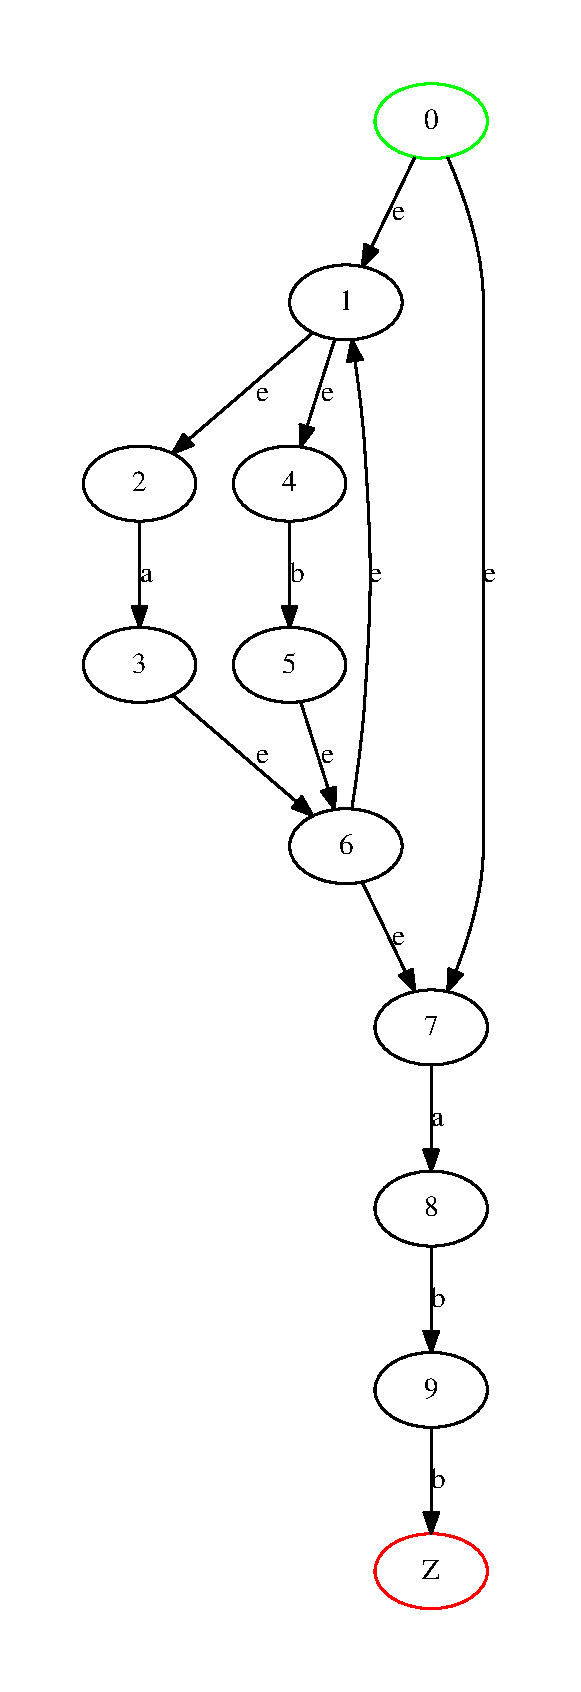
\includegraphics[scale = 0.5]{automata1.pdf}
 \caption{Autómata Finito No Determinista}
\end{figure}

\begin{figure}[h]
 \centering
 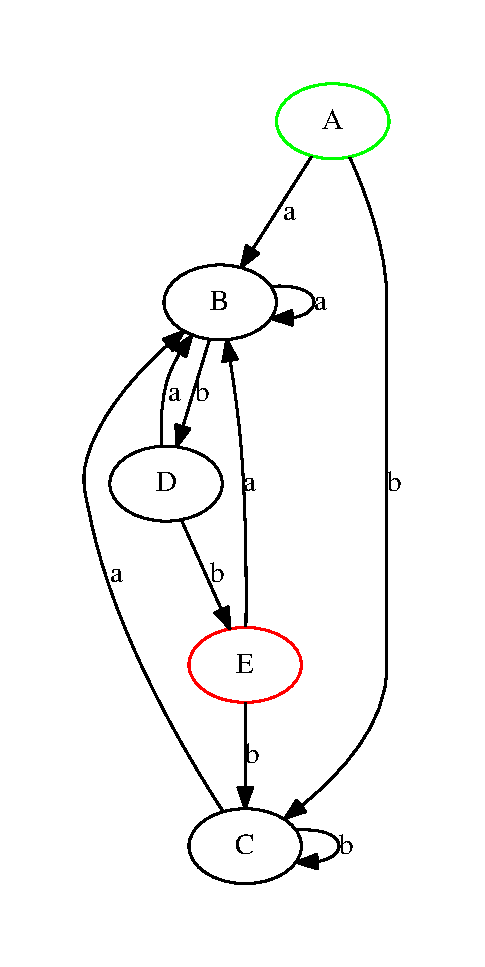
\includegraphics[scale = 0.5]{resultado.pdf}
 \caption{Resultado: Autómata Finito Determinista}
\end{figure}




\end{document}
